\documentclass[t]{beamer}
\usetheme{Copenhagen}
\setbeamertemplate{headline}{} % remove toc from headers
\beamertemplatenavigationsymbolsempty

\usepackage{amsmath, tikz, bm, tkz-euclide,pgfplots}
\pgfplotsset{compat = 1.16}
\usetkzobj{all}

\title{Equations and Inequalities}
\author{}
\date{}

\AtBeginSection[]
{
  \begin{frame}
    \frametitle{Objectives}
    \tableofcontents[currentsection]
  \end{frame}
}

\begin{document}

\begin{frame} 
\maketitle
\end{frame}

\section{Solve linear equations and check solutions.}

\begin{frame}{Solving Equations}
When solving an equation, our goal is to get the variable, usually $x$, alone on one side of the equal sign.	\newline\\	\pause

To do this, we use \alert{reverse order of operations}:	\newline\\	\pause
\begin{enumerate}
	\item<+-> Undo any addition or subtraction. 
	\item<+-> Undo any multiplication or division.
	\item<+-> Undo any exponents.
	\item<+-> Get rid of parentheses.
\end{enumerate}
\end{frame}

\begin{frame}{Checking Your Answer}
You can make sure your answer is correct by {\color{blue}\textbf{plugging it in}} to the original problem and seeing if the left side and right side are equal.
\end{frame}

\begin{frame}{Example 1}
Solve each of the following. Round to 2 decimal places.	\newline\\
(a) \quad $3x + 4 = 16$
\begin{align*}
\onslide<2->{3x+4 &= 16 &} \\[6pt]
\onslide<3->{3x &= 12 &\text{subtract 4}} \\[6pt]
\onslide<4->{x &= 4 &\text{divide by 3}}
\end{align*}
\onslide<5->{Check $x = 4$:}
\begin{align*}
\onslide<6->{3(4) + 4 &= 16?} \\
\onslide<7->{16 &= 16}
\end{align*}
\onslide<8->{\[x=4\]}
\end{frame}

\begin{frame}{Example 1}
(b) \quad $-2x-9=17-x$ 
\begin{align*}
\onslide<2->{-2x-9&=17-x &} \\[6pt]
\onslide<3->{-1x - 9 &= 17 &\text{add $x$}} \\[6pt]
\onslide<4->{-1x &= 26 &\text{add 9}}	\\[6pt]
\onslide<5->{x &= -26 &\text{divide by $-1$}}
\end{align*}
\onslide<6->{Check $x = -26$:}
\begin{align*}
\onslide<7->{-2(-26)-9 &= 17 - (-26)?} \\[6pt]
\onslide<8->{43 &= 43}
\end{align*}
\onslide<9->{\[x=-26\]}
\end{frame}

\begin{frame}{Example 1}
(c) \quad $\frac{1}{2}x + 3 = \frac{2}{5}x$
\begin{align*}
\onslide<2->{\frac{1}{2}x + 3 &= \frac{2}{5}x &} \\[8pt]
\onslide<3->{3 &= -\frac{1}{10}x &\text{subtract $\frac{1}{2}x$}} \\[8pt]
\onslide<4->{-30 &= x &\text{divide by $-\frac{1}{10}$}}
\end{align*}
\onslide<5->{Check $x=-30$:}
\begin{align*}
\onslide<6->{\frac{1}{2}(-30)+3 &= \frac{2}{5}(-30)?} \\[8pt]
\onslide<7->{-12 &= -12}
\end{align*}
\onslide<8->{\[x = -30\]}
\end{frame}

\begin{frame}{Example 1}
(d) \quad $2.1x - 7 = 23.83$
\begin{align*}
\onslide<2->{2.1x - 7 &= 23.83 &} \\[6pt]
\onslide<3->{2.1x &= 30.83 &\text{add 7}} \\[6pt]
\onslide<4->{x &\approx 14.68 &\text{divide by 2.1}}
\end{align*}
\onslide<5->{Check $x \approx 14.68$:}
\begin{align*}
\onslide<6->{2.1(14.68) - 7 &\approx 23.83?} \\[6pt]
\onslide<7->{23.828 &\approx 23.83}
\end{align*}
\onslide<8->{\[x \approx 23.83\]}
\end{frame}

\begin{frame}{Example 1}
(e) \quad $2(x-10) = 4(x-5)-2x$
\begin{align*}
\onslide<2->{2(x-10) &= 4(x-5)-2x &} \\[6pt]
\onslide<3->{2x-20 &= 4x-20 - 2x &\text{distribute}} \\[6pt]
\onslide<4->{2x-20 &= 2x-20 &\text{combine like terms on the right}} \\[6pt]
\onslide<5->{-20 &= -20 &\text{subtract $2x$ from both sides}}
\end{align*}
\onslide<6->{True statement, so $x = \text{all real numbers, or }\mathbb{R}$}
\end{frame}

\begin{frame}{Example 1}
(f) \quad $3(x+4)+3x = 2(3x+5)-2$
\begin{align*}
\onslide<2->{3(x+4)+3x &= 2(3x+5)-2 &} \\[6pt]
\onslide<3->{3x+12+3x &= 6x+10-2 &\text{distribute}} \\[6pt]
\onslide<4->{6x+12 &= 6x+8 &\text{combine like terms}} \\[6pt]
\onslide<5->{12 &= 8 &\text{subtract $6x$ from both sides}}
\end{align*}
\onslide<6->{False statement, so $x = \text{No solution, or } \varnothing$}
\end{frame}

\begin{frame}{Visual Way to Check Answers}
Another useful way to help check your answers is to graph the left side of the equation, as well as the right side. \newline\\	\pause

The solution is the $x$-coordinate of their \alert{intersection point}.	\newline\\	\pause

For ``no solution'' answers, the graphs will \textbf{never intersect}. \newline\\	\pause

For ``all real numbers'' answers, the graphs will be \textbf{one in the same}.
\end{frame}

\begin{frame}{Visual Way to Check Answers}
The graphs of $y = 3x+4$ and $y=16$ are shown below:	\newline\\
\begin{center}
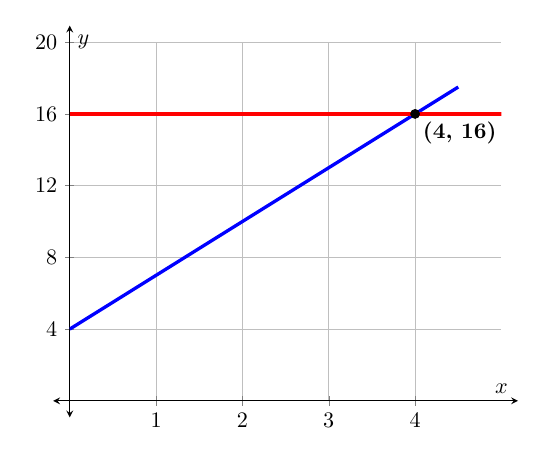
\begin{tikzpicture}[scale=0.8]
    \begin{axis}
    [
    xlabel = $x$,
    ylabel = $y$,
    axis lines = middle,
    axis line style={stealth-stealth},
    axis line style={shorten >=-7.5pt, shorten <=-7.5pt},
    xmin = 0, xmax = 5,
    ymin = 0, ymax = 20,
    ystep = 4,
    xtick = {-4,-3,...,4},
    ytick = {4,8,...,20},
    grid,
    every axis x label/.style = {at = {(ticklabel* cs:1)}, anchor = south},
    every axis y label/.style = {at = {(ticklabel* cs:1)}, anchor = west}
    ]
    \addplot[domain = 0:4.5, samples = 200, line width = 1.5, smooth, color=blue]{3*x+4};
    \addplot[domain = 0:5, samples = 200, line width = 1.5, smooth, color=red] {16};
    \addplot [mark = *] coordinates {(4, 16)} node [below right] {\textbf{(4, 16)}};
    \end{axis}
    \end{tikzpicture}
\end{center}
\end{frame}


\section{Solve and graph inequalities on a number line.}


\begin{frame}{Solving Inequalities}
Solving inequalities is a lot like solving equations.	\newline\\	\pause

The biggest difference is that {\color{blue}\textbf{inequalities typically give you an infinite number of solutions.}}	\newline\\	\pause

For instance, there are an infinite number of values that you can substitute into $x$ for $x > -4$ to make it true.
\end{frame}

\begin{frame}{Visual Solutions to Inequalities}
Since we can't list every possible solution, we can shade a region on a number line to represent this solution.	\newline\\	\pause
\begin{center}
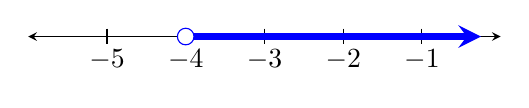
\begin{tikzpicture}
	\draw [<->, > = stealth] (-6,0) -- (-0,0);
	\foreach \x in {-5,-4,-3,-2,-1}
	\draw (\x, 0.1) -- (\x, -0.1);
	\foreach \x in {-5,-4,-3,-2,-1}
	\node at (\x, -0.3) {$\x$};
	\draw [->, color = blue, line width = 2.5, >=stealth] (-3.92,0) -- (-0.25,0);
	\draw [color = blue, fill=white] (-4,0) circle (3pt);
\end{tikzpicture}
\end{center}
\end{frame}

\begin{frame}{Summary of Graphing Inequalities}
If your variable is on the \alert{left side} when graphing an inequality, you can use the following table to help you graph:	\newline\\
\begin{center}
\setlength{\extrarowheight}{4pt}
\begin{tabular}{c|c|c}  
\textbf{Expression}	&	\textbf{Circle}	&	\textbf{Shade}	\\
\hline
$x<$					&	Open				& 	Left		\\[4pt]
\hline
$x>$					&	Open				&	Right	\\[4pt]
\hline
$x \leq$				&	Closed			&	Left		\\[4pt]
\hline
$x \geq$				&	Closed			&	Right	\\[4pt]
\end{tabular}
\end{center}
\end{frame}

\begin{frame}{Example 2}
Graph each of the following on a number line.	\newline\\
\quad $x < 2$	\newline\\	
\begin{center}
\onslide<2->{
	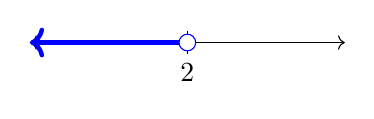
\begin{tikzpicture}
	\draw[<->] (-2,0) -- (2,0);
	\draw (0,0.15) -- (0,-0.15) node [below] {$2$};
	\onslide<3->{\draw[color=blue,fill=white] (0,0) circle [radius=3pt];}
	\onslide<4->{\draw[->,color=blue,ultra thick, shorten <= 3pt] (0,0) -- (-2,0);}
	\end{tikzpicture}	
}
\end{center}
\end{frame}

\begin{frame}{Solving Inequalities}
With solving inequalities, you must remember to flip the inequality sign if you multiply or divide {\color{blue}\textbf{both sides}} by a \alert{negative number}.
\end{frame}

\begin{frame}{Example 3}
Solve and graph each.	\newline\\
(a) \quad $3x - 5 > -17$
\begin{align*}
\onslide<2->{3x-5 &> -17 &}	\\[6pt]
\onslide<3->{3x &> -12 &\text{add 5}} \\[6pt]
\onslide<4->{x &> -4 &\text{divide by 3}} \\[6pt]
\end{align*}
\begin{center}
\onslide<5->{
	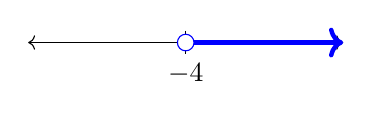
\begin{tikzpicture}
	\draw[<->] (-2,0) -- (2,0);
	\draw (0,0.15) -- (0,-0.15) node [below] {$-4$};
	\onslide<6->{\draw[color=blue,fill=white] (0,0) circle [radius=3pt];}
	\onslide<7->{\draw[->,color=blue,ultra thick, shorten <= 3pt] (0,0) -- (2,0);}
	\end{tikzpicture}
}
\end{center}
\end{frame}

\begin{frame}{Example 3}
(b) \quad $2(x+4)-5 > 2x + 3$
\begin{align*}
\onslide<2->{2(x+4)-5 &> 2x+3 &} \\[6pt]
\onslide<3->{2x+8-5 &> 2x+3 &\text{distribute the 2}} \\[6pt]
\onslide<4->{2x+3 &> 2x + 3 &\text{combine like terms}} \\[6pt]
\onslide<5->{3 &> 3 &\text{subtract $2x$ from both sides}}
\end{align*}
\onslide<6->{False statement. \quad}
\onslide<7->{No Solution ($\varnothing$)} 
\begin{center}
\onslide<8->{
	\begin{tikzpicture}
	\draw[<->] (-2,0) -- (2,0);
	\end{tikzpicture}
}
\end{center}
\end{frame}

\begin{frame}{Example 3}
(c) \quad $3(x+1) \geq 3x + 2$
\begin{align*}
\onslide<2->{3(x+1) &\geq 3x+2 &} \\[6pt]
\onslide<3->{3x+3 &\geq 3x+2 &\text{distribute}} \\[6pt]
\onslide<4->{3 &\geq 2 &\text{subtract $3x$ from both sides}}
\end{align*}
\onslide<5->{True statement. \quad}
\onslide<6->{All real numbers ($\mathbb{R}$)}
\begin{center}
\onslide<7->{
	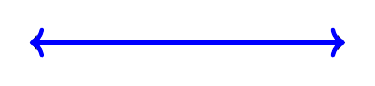
\begin{tikzpicture}
	\draw[<->] (-2,0) -- (2,0);
	\onslide<8->{\draw[<->,color=blue,ultra thick] (-2,0) -- (2,0);}
	\end{tikzpicture}
}
\end{center}
\end{frame}

\end{document}
